In this section we introduce a system of
risk groups, flows between them, and equations
which can be used to describe turnover
in deterministic compartmental epidemic models.
% ==================================================================================================
\subsection{Notation}
Consider a population divided into $G$ risk groups.
We denote the number of individuals in risk group $i \in [1, \dots, G]$ as $x_i$
and the set of all risk groups as $\bm{x} = \{x_1, \dots, x_G\}$.
The total population size is $N = \sum_i {x_i}$,%
\footnote{Here, as in many models, ``total population'' actually represents
  a subset of the population with a given duration in the model --
  e.g. an age-constrained range.}
and the proportion of the total population that each group represents
is denoted as $\hat{x}_i = x_i / N$.
We do not consider stratification of age groups.
Individuals enter the model at a rate $\nu$ per year,
and exit at a rate $\mu$ per year.
However, the proportion of individuals entering into group $i$ from outside the model
may be different from
the proportion of individuals currently in group $i$ in the model ($\hat{x}_i$).
Therefore, we distinguish these proportions
and denote the proportion entering into group $i$ as $\hat{e}_i$.
For example, a higher proportion of youth (individuals entering the model, $\hat{e}_i$)
may engage in high-risk sexual behaviour,
as compared to the population overall ($\hat{x}_i$).
It will later be shown how rates of turnover can maintain such a system at equilibrium.
% The number of entrants into group $i$ is therefore given by
% $\nu N \hat{e}_i$.
% This assumption then implies then implies the existence of
% a ``source'' population $\bm{e} = \{e_1, \dots, e_G\}$,
% from which model entrants originate.
% The size of this population is then assumed to be the same as $\bm{x}$ ($\sum_i e_i = N$)
% so that the entry rate $\nu$ can be used in the usual way,
% as a proportion of $N$.
\par
Turnover transitions may occur between any two groups, in either direction;
therefore we denote the turnover rates as a $G \times G$ matrix $\phi$.
The element $\phi_{ij}$ corresponds to the proportion of individuals in group $x_i$
who move from group $x_i$ to group $x_j$ each year.
An example matrix is given in Eq.~(\ref{eq:phi}),
where we write the diagonal elements as $*$ since they represent
transitions from a group to itself, which are inconsequential.
\begin{equation}\label{eq:phi}
\phi = \left[\begin{array}{cccc}
	         *          & x_1  \rightarrow x_2 & \cdots & x_1 \rightarrow x_G \\[0.5em]
	x_2 \rightarrow x_1 &          *           & \cdots & x_2 \rightarrow x_G \\[0.5em]
	      \vdots        &        \vdots        & \ddots &       \vdots        \\[0.5em]
	x_G \rightarrow x_1 & x_G \rightarrow x_2  & \cdots &          *
\end{array}\right]
\end{equation}
These transition flows and the associated rates
are also shown for $G = 3$ in Figure~\ref{fig:system}.
\begin{figure}
  \centering
  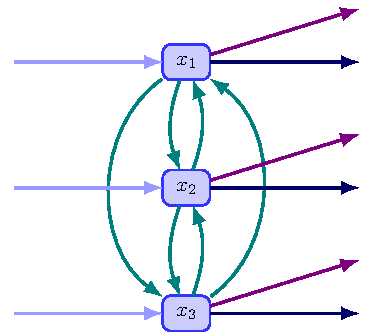
\includegraphics[width=0.5\linewidth]{turnover-system}
  \caption{System of states and flows between them for $G = 3$}
  \label{fig:system}
\end{figure}
% ==================================================================================================
\subsection{Parameterization}\label{ss:params}
Next, we consider the goal of constructing a system like the one introduced above
which reflects the risk group dynamics observed in a specific context.
We assume that the relative sizes of the risk groups in the model ($\bm{\hat{x}}$)
are already known, and should remain constant over time.
Thus, what remains is to estimate the values of the parameters:
$\nu$, $\mu$, $\bm{\hat{e}}$, and $\phi$,
using commonly available sources of data.
% --------------------------------------------------------------------------------------------------
\subsubsection{Total Population Size}\label{sss:params-nu-mu}
The total population size $N(t)$ is related to
the rates of population entry $\nu(t)$ and exit $\mu(t)$.
We consider variation in rate of entry across risk groups via $\bm{\hat{e}}$,
and we do not stratify the rate of exit by activity group
(disease-attributable death is assumed to be negligible for now).
Therefore, we can assume that $\nu$ and $\mu$ do not vary across risk groups,
allowing these rates to be estimated independent of
$\bm{\hat{x}}$, $\bm{\hat{e}}$, and $\phi$.
\par
The difference between entry and exit rates
defines the rate of population growth:
\begin{equation}\label{eq:growth-G}
\mathcal{G}(t) = \nu(t) - \mu(t) 
\end{equation}
The total population may then be defined using an initial population size $N_0$ as:
\begin{equation}\label{eq:growth-vary}
  N(t) = N_0 \exp{\left(\int_{0}^{\,t}{\log\big(1+\mathcal{G}(\tau) \big)d\tau}\right)}
\end{equation}
which, for constant growth, simplifies to the familiar expression:
\begin{equation} \label{eq:growth-const}
  N(t) = N_0 {(1 + \mathcal{G})}^{t}
\end{equation}
In most cases, demographic data will be available
on the total size of the population over time $N(t)$,
allowing Eqs.~(\ref{eq:growth-vary})~and~(\ref{eq:growth-const})
to be used to estimate $\mathcal{G}(t)$.
\par
If we assume that the population size is constant, then $\mathcal{G}(t) = 0$ and $\nu(t) = \mu(t)$.
However, this is generally not a good assumption, 
as it does not reflect the positive population growth observed in many contexts.
We will also later show that this assumption may impact epidemic dynamics.
Another approach is to fix $\mathcal{G}$ at a constant value.
This value can be estimated via Eq.~(\ref{eq:growth-const})
using any two values of $N(t)$, separated by a time interval $\tau$:
\begin{equation}
\mathcal{G}_{\tau} = {\frac{N(t+\tau)}{N(t)}}^{\frac{1}{\tau}} -1
\end{equation}
For contexts with variability in $\mathcal{G}$ over time,
this process can be repeated for consecutive time intervals,
and the complete function $\mathcal{G}(t)$ approximated piecewise by constant values.
This approach is generally more feasible than exact solutions using Eq.~(\ref{eq:growth-vary}),
and can reproduce $N(t)$ accurately for small enough intervals $\tau$,
such as one year.
\par
Now, a given value of $\mathcal{G}(t)$ does not imply any particular
values of $\nu(t)$ or $\mu(t)$,
since any choice of $\mu(t)$ can be compensated by an appropriate choice of $\nu(t)$,
and vice versa, as in Eq.~(\ref{eq:growth-G}).
However, it is common to assume a constant duration of individuals in the model $\delta(t)$,
which is related to the rate of exit by:
\begin{equation} \label{eq:duration-model}
\delta(t) = \mu^{-1}(t)
\end{equation}
Such a duration should reflect the demographic data used to define $N(t)$,
as well as the epidemiological data used to inform other model parameters.
For example, an age range of 15~to~50 years implies a duration in the model of $\delta = 35$ years.
The duration may also vary with time to reflect contextual changes to all-cause mortality.
In any case, $\mu(t)$ can then be defined as $\delta^{-t}(t)$
following Eq.~(\ref{eq:duration-model}),
and $\nu(t)$ defined as $\mathcal{G}(t) - \mu(t)$
following Eq.~(\ref{eq:growth-G}).
% --------------------------------------------------------------------------------------------------
\subsubsection{Turnover}\label{sss:params-turnover}
Next, we present methods for resolving
the distribution of individuals entering the risk model $\bm{\hat{e}}(t)$ and
the rates of turnover $\phi(t)$,
assuming that entry and exit rates $\nu(t)$ and $\mu(t)$ are known.
Similar to above, we first formulate the problem as a system of equations.
Then, we explore the data and assumptions which can be leveraged
to solve for the values of parameters in the system.
The $(t)$ notation is omitted throughout this section for clarity,
though time-varying parameters can be estimated by
repeating the necessary calculations for each $t$.
\par
Depending on the number of risk groups $G$,
there are $G$ unknown elements in $\bm{\hat{e}}$ and $G(G-1)$ unknown elements in $\phi$.
We collect these unknowns in the vector
$\bm{\theta} = \left[\bm{\hat{e}}, \bm{y}\right]$,
where $\bm{y} = \mathrm{vec}_{i \ne j}(\phi)$.
For example, for $G = 3$, the vector $\bm{\theta}$ is defined as:
\begin{equation}
\bm{\theta} = \left[
\begin{array}{ccccccccc}
\hat{e}_1 & \hat{e}_2 & \hat{e}_3 & \phi_{12} & \phi_{13} & \phi_{21} & \phi_{23} & \phi_{31} & \phi_{32}
\end{array}\right]
\end{equation}
The crux of this framework is then to define a linear system of equations
which uniquely determine the elements of $\bm{\theta}$:
\begin{equation}\label{eq:system-matrix}
\bm{b} = A \thinspace \bm{\theta}
\end{equation}  
where $A$ is a $M \times G^2 $ matrix
and $\bm{b}$ is a $M$-length vector.
That is, each row in $A$ and $\bm{b}$ specifies
an assumed relationship involving elements of
$\bm{\hat{e}}$ and $\phi$.
Given a sufficient number $M = G^2$ of unique constraints,
the parameters can be calculated algebraically using $\bm{\theta} = A^{-1}\bm{b}$.
Some examples of constraints are explored below.
% --------------------------------------------------------------------------------------------------
\paragraph{Constant Group Size}
First, we define the ``conservation of mass'' equation for group $x_i$,
wherein the rate of change of the group
is defined as the sum of flows in\,/\,out of the group:
\begin{equation}\label{eq:mass-balance}
\frac{d}{dt}x_i
= \nu \thinspace e_i + \sum_{j}{\phi_{ji} \thinspace x_j}
- \mu \thinspace x_i - \sum_{j}{\phi_{ij} \thinspace x_i}
\end{equation}
While Eq.~(\ref{eq:mass-balance}) is written in terms of
absolute population sizes $\bm{x}$ and $\bm{e}$,
it is equivalent to divide through by $N$,
yielding a system in terms of
proportions $\bm{\hat{x}}$ and $\bm{\hat{e}}$,
which can be more useful, since $N$ need not be known.
% not sure if there is additional normalization needed, actually
If we assume that the average proportions of each group $\hat{x}_i$ is constant over time,
then the desired rate of change for risk group $i$
will be equal to the growth of the risk group, $\mathcal{G} x_i$.
Substituting this into Eq.~(\ref{eq:mass-balance}),
and simplifying yields:
\begin{equation}\label{eq:system}
\nu \thinspace x_i
= \nu \thinspace e_i + \sum_{j}{\phi_{ji} \thinspace x_j}
- \sum_{j}{\phi_{ij} \thinspace x_i}
\end{equation}
Factoring the left and right hand sides in terms of $\bm{\hat{e}}$ and $\phi$,
we obtain $G$ unique constraints.
For $G = 3$, this yields the following 3 rows as the basis of $\bm{b}$ and $A$:
\begin{equation}\label{eq:b-A-basis}
\bm{b} = \left[\begin{array}{c}
\nu x_1 \\ \nu x_2 \\ \nu x_3
\end{array}\right];\qquad
A = \left[\begin{array}{ccccccccc}
 \nu  & \cdot & \cdot & -x_1  & -x_1  &  x_2  & \cdot &  x_3  & \cdot \\
\cdot &  \nu  & \cdot &  x_1  & \cdot & -x_2  & -x_2  & \cdot &  x_3  \\
\cdot & \cdot &  \nu  & \cdot &  x_1  & \cdot &  x_2  & -x_3  & -x_3  \\
\end{array}\right] 
\end{equation}
These $G$ constraints are necessary to ensure risk groups do not change size over time.
However, to obtain a unique solution,
we still need an additional $G(G-1)$ constraints.
For $G = 3$, this corresponds to 6 additional constraints.
% --------------------------------------------------------------------------------------------------
\paragraph{Specified Elements}
The simplest type of additional constraint is to
directly specify individual elements in $\bm{\hat{e}}$ or $\phi$.
This constraint may be appended to $\bm{b}$ and $A$ using indicator encoding:
with $b_k$ as the specified value and $A_k = [0,\dots,1,\dots,0]$ as the indicator vector.
For example, for $G = 3$, if it is known that 20\% of individuals
enter directly into risk group $x_1$ upon entry into the model ($\hat{e}_1 = 0.20$),
then $\bm{b}$ and $A$ can be augmented with:
\begin{equation}
\bm{b}' = \left[\begin{array}{c} 0.20 \end{array}\right];\qquad
A' = \left[\begin{array}{ccccccccc}
1 & \cdot & \cdot & \cdot & \cdot & \cdot & \cdot & \cdot & \cdot \\
\end{array}\right] 
\end{equation}
If we do not want any turnover from group $i$ to group $j$,
then this approach can also be used to set $\phi_{ij} = 0$.
Note that the elements of $\bm{\hat{e}}$ must sum to one.
Therefore, specifying all elements in $\bm{\hat{e}}$
will only provide $G-1$ additional constraints,
as the last element is redundant.
This relationship is implicit in Eq.~(\ref{eq:b-A-basis}),
so it is not necessary to supply a constraint $1 = \sum_{i} \hat{e}_i$.
Similar redundancies or inconsistencies can emerge for constraints on $\phi$, as noted below.
% --------------------------------------------------------------------------------------------------
\paragraph{Group Duration}
Another useful constraint can be derived from
the average duration of individuals in a risk group.
This duration $\delta_i$ is defined as the inverse of all efferent flow rates:
\begin{equation}\label{eq:duration-group}
\delta_i = {\bigg(\mu + \sum_{j}{\phi_{ij}}\bigg)}^{-1}
\end{equation}
Average durations could be derived from survey data, including for key populations, % SS: define KP
or they could be assumed.
These values can be used to define constraints on $\phi$ by
rearranging Eq.~(\ref{eq:duration-group}) to yield:
${\delta_{i}}^{-1} - \mu = \sum_{j}{\phi_{ij}}$.
For example, if for $G = 3$,
the average duration in group $x_1$ is known to be $\delta_1 = 5$ years,
then $\bm{b}$ and $A$ can be augmented with:
\begin{equation}
\bm{b}' = \left[\begin{array}{c}
{5}^{-1} - \mu
\end{array}\right];\qquad
A' = \left[\begin{array}{ccccccccc}
\cdot & \cdot & \cdot & 1 & 1 & \cdot & \cdot & \cdot & \cdot \\
\end{array}\right]
\end{equation}
As noted above, redundancies can emerge
when constraining turnover rates $\phi$ via duration $\delta_i$.
Namely, specifying all efferent flow rates $\phi_{ij}$ for one group $i$
will fully determine the duration in the group $\delta_i$.
In general, each constraint which is not redundant will increase the rank of $A$ by one,
and $A$ must be full rank ($G^2$) to uniquely determine the parameters in $\bm{\theta}$.
% --------------------------------------------------------------------------------------------------
\paragraph{Turnover Balance}
We present one final constraint here.
We can assume that
the absolute number of individuals moving between two risk groups is
related by a ratio $\frac{r_i}{r_j}$ so that:
$\phi_{ij} x_{i} r_{i} = \phi_{ji} x_{j} r_{j}$.
This helps constrain $\phi_{ij}$ and $\phi_{ji}$.
For example, for $G = 3$,
if we assume that the number of individuals moving between groups $x_1$ and $x_2$
is related by $\frac{3}{2}$,
then $\bm{b}$ and $A$ can be augmented with:
\begin{equation}
\bm{b}' = \left[\begin{array}{c}
0
\end{array}\right];\qquad
A' = \left[\begin{array}{ccccccccc}
\cdot & \cdot & \cdot & 3 x_1 & \cdot & -2 x_2 & \cdot & \cdot & \cdot \\
\end{array}\right] 
\end{equation}
If we assume that the absolute number of individuals moving between the groups is equal,
then simply $\frac{r_i}{r_j} = 1$.
Again, care should be taken to avoid redundancies and inconsistencies with other constraints.
%% JK: I feel this should be elaborated on,
%% but its honestly very difficult to summarize the situations where this occurs.
% --------------------------------------------------------------------------------------------------
\paragraph{Minimization}
Lastly, we can avoid specifying a complete set of constraints on $\bm{\theta}$
($A$ can be less than full rank)
if the problem is posed as a minimization problem, namely:
\begin{equation}\label{eq:system-optimize}
\bm{\theta}^{*} = {\arg \min}
\thinspace f(\bm{\theta}),
\quad \textrm{subject to:}
\enspace\bm{b} = A\thinspace\bm{\theta};
\enspace\bm{\theta} \ge 0
\end{equation}
where $f$ is a function which globally constrains $\bm{\theta}$,
such as: ${\left|\left| \,\cdot\, \right|\right|}_2$.
That is, when a sufficient number of assumptions cannot be made about $\bm{\hat{e}}$ and $\phi$
to yield a unique solution,
this approach can be used to find the smallest values of $\bm{\hat{e}}$ and $\phi$
which satisfy the given constraints.
Numerical solutions to such problems are widely available,
such as the Non-Negative Lease Squares solver \citep{Lawson1995}.%
\footnote{The \textsc{nnls} solver is available in Python:
   \href{https://docs.scipy.org/doc/scipy/reference/generated/scipy.optimize.nnls.html}
{\texttt{https://docs.scipy.org/doc/scipy/reference/generated/scipy.optimize.nnls.html}}.}
%% JK: may want to add a paragraph on inconsistent systems (no true solution):
%% how to identify them and what to do about them.
% ==================================================================================================
\subsection{Previous Approaches}
While most models have included population growth,
many have not included risk heterogeneity within age-sex groups,
and still fewer have simulated turnover among risk groups.
These three major features about risk group dynamics and the associated assumptions
are summarized in Box~\ref{box:assumptions}.
In each case, option (b) typically represents the more plausible assumption.
Experiment 1 in the next section
aims to illustrate the potential implications of assuming option (a).
\begin{floatbox}
  \caption{Common assumptions regarding the dynamics of risk groups}
  \label{box:assumptions}
  \begin{fboxed}
  \begin{enumerate}[leftmargin=1em]
    \item\label{ass:risk-groups}\textbf{Risk Groups:}
    Major demographic groups are stratified by risk of HIV acquisition.
    \begin{enumerate}
      \item\label{ass:risk-groups-no}\textbf{No:} $\G = 1$;
      Major demographic groups are homogeneous in risk of HIV acquisition.
      \item\label{ass:risk-groups-yes}\textbf{Yes:} $\G > 1$;
      Heterogeneity in risk of HIV acquisition within major demographic groups is considered.
    \end{enumerate}
    \item\label{ass:turnover}\textbf{Turnover:}
    Individuals may move between risk groups.
    \begin{enumerate}
      \item\textbf{No:} $\zeta = 0$;
      Individuals do not move between risk groups.
      \item\textbf{Constant:} $\zeta > 0$;
      Individuals move between risk groups at a constant rate.
%      \item\textbf{Dynamic:} $\zeta = f$;
%      Individuals move between risk groups in dynamically.
    \end{enumerate}
    \item\label{ass:pop-growth}\textbf{Population Growth:}
    Increase in the total $\N$ over time.
    \begin{enumerate}
      \item\textbf{No:} $\nu = \mu$;
      Population size $\N$ is constant.
      \item\textbf{Yes:} $\nu > \mu$;
      Population size $\N$ increases, at some constant or data-driven rate.
    \end{enumerate}
  \end{enumerate}
\end{fboxed}

\end{floatbox}
\par
Among those works which have considered risk groups and turnover among them,
implementations have varied widely.
In a $G = 2$ system,
\citet{Stigum1994} use a parameter $\kappa$ to define
the rate of movement of individuals from a core group into the remaining population,
which is balanced by an equal number of individuals moving in the opposite direction.
Considered through the proposed framework,
this defines a unique system through assuming:
a \emph{specified element} $\kappa = \phi_{12}$,
\emph{constant group size}, and \emph{balanced turnover}.
\citet{Henry2015} employ the same assumptions for another $G = 2$ system,
but define a ``re-selection rate'' $\omega$ to control
the relative rate of turnover, so that
$\phi_{12} = \omega \hat{x}_{2}$ and $\phi_{21} = \omega \hat{x}_{1}$.
In a $G = 3$ system,
\citet{Eaton2014} use a parameter $\Psi$ to define the rate of movement from
high-to-low, high-to-medium, and medium-to-low risk groups each year,
but assume no transitions in the opposite direction.
Thus, all six elements of $\phi$ are \emph{specified},
while \emph{constant group sizes} are ensured by computing
the required distribution of model entrants $\bm{\hat{e}}$
via equation [S12] in the Supplemental Information.
\par
The $G = 7$ system used by
\citet{Boily2015} is highly contextual, and
includes four high-risk groups which transition to specific low-risk groups
(e.g. from ``high-/low-volume sex work'' to ``formerly engaged in sex work'').
The turnover matrix $\phi$ is then completely \emph{specified} (though notably sparse)
using several assumptions about \emph{group durations}.
The distribution of risk groups among individuals entering the model $\bm{\hat{e}}$
is also \emph{specified},
leaving the distribution of risk groups among individuals in the model $\bm{\hat{x}}$
as the only free parameters.
For this reason, a 100-year ``burn-in'' period is required
to equilibrate risk-group sizes before introduction of HIV in the model.
Note that this approach is not perfectly compatible with the framework presented here,
since we assume \emph{constant group sizes}
as the basis for the system in Eq.~(\ref{eq:b-A-basis}),
and exclude $\bm{\hat{x}}$ from the vector of free parameters $\bm{\theta}$.
However, by relaxing these constraints,
it should be possible to formulate even the implementation by \citet{Boily2015}
in terms of the proposed framework.
\par
In sum, the framework for modelling turnover presented here aims to generalize
all previous implementations.
In so doing, we hope to clarify the requisite assumptions,
dependencies on epidemiological data,
and relationships between previous approaches.
In Experiments 2 and 3, we leverage this framework to explore
the potential influences of turnover on epidemics.